% This is part of Un soupçon de mathématique sans être agressif pour autant
% Copyright (c) 2013
%   Laurent Claessens
% See the file fdl-1.3.txt for copying conditions.

% Ce fichier est celui pour les secondes.

Distribuer aux élèves le dessin de la page suivante et en discuter.
\begin{center}

           \ifpdf
            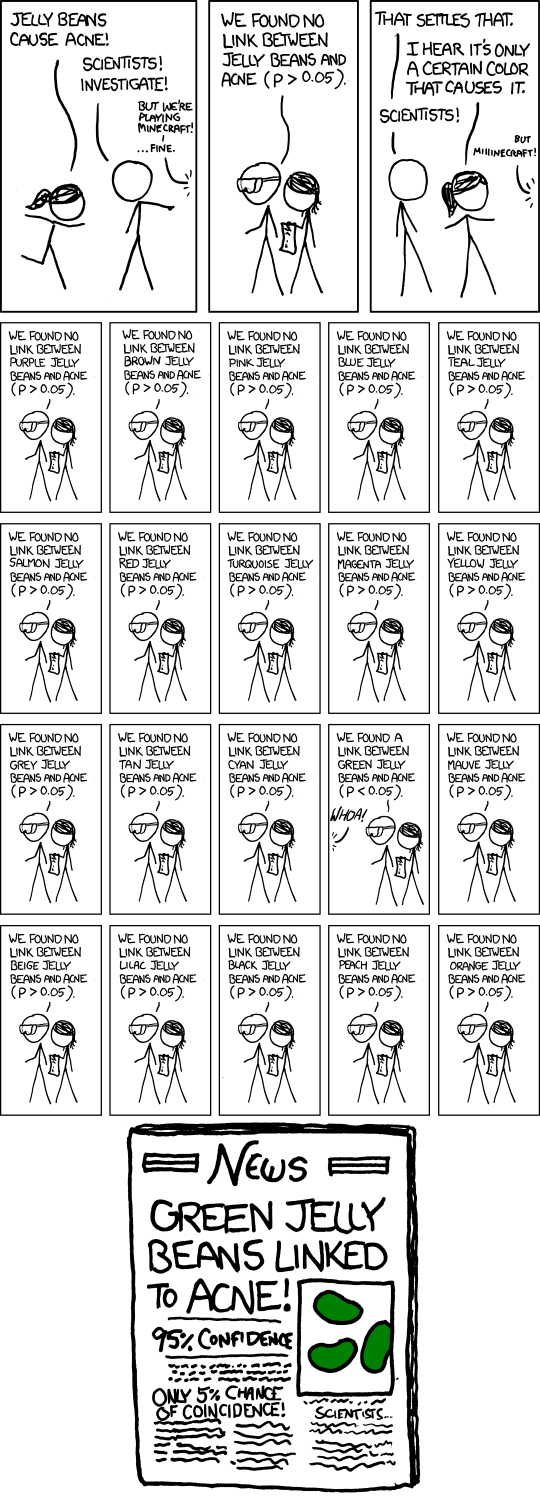
\includegraphics[width=8cm]{significant.png}
        \else
            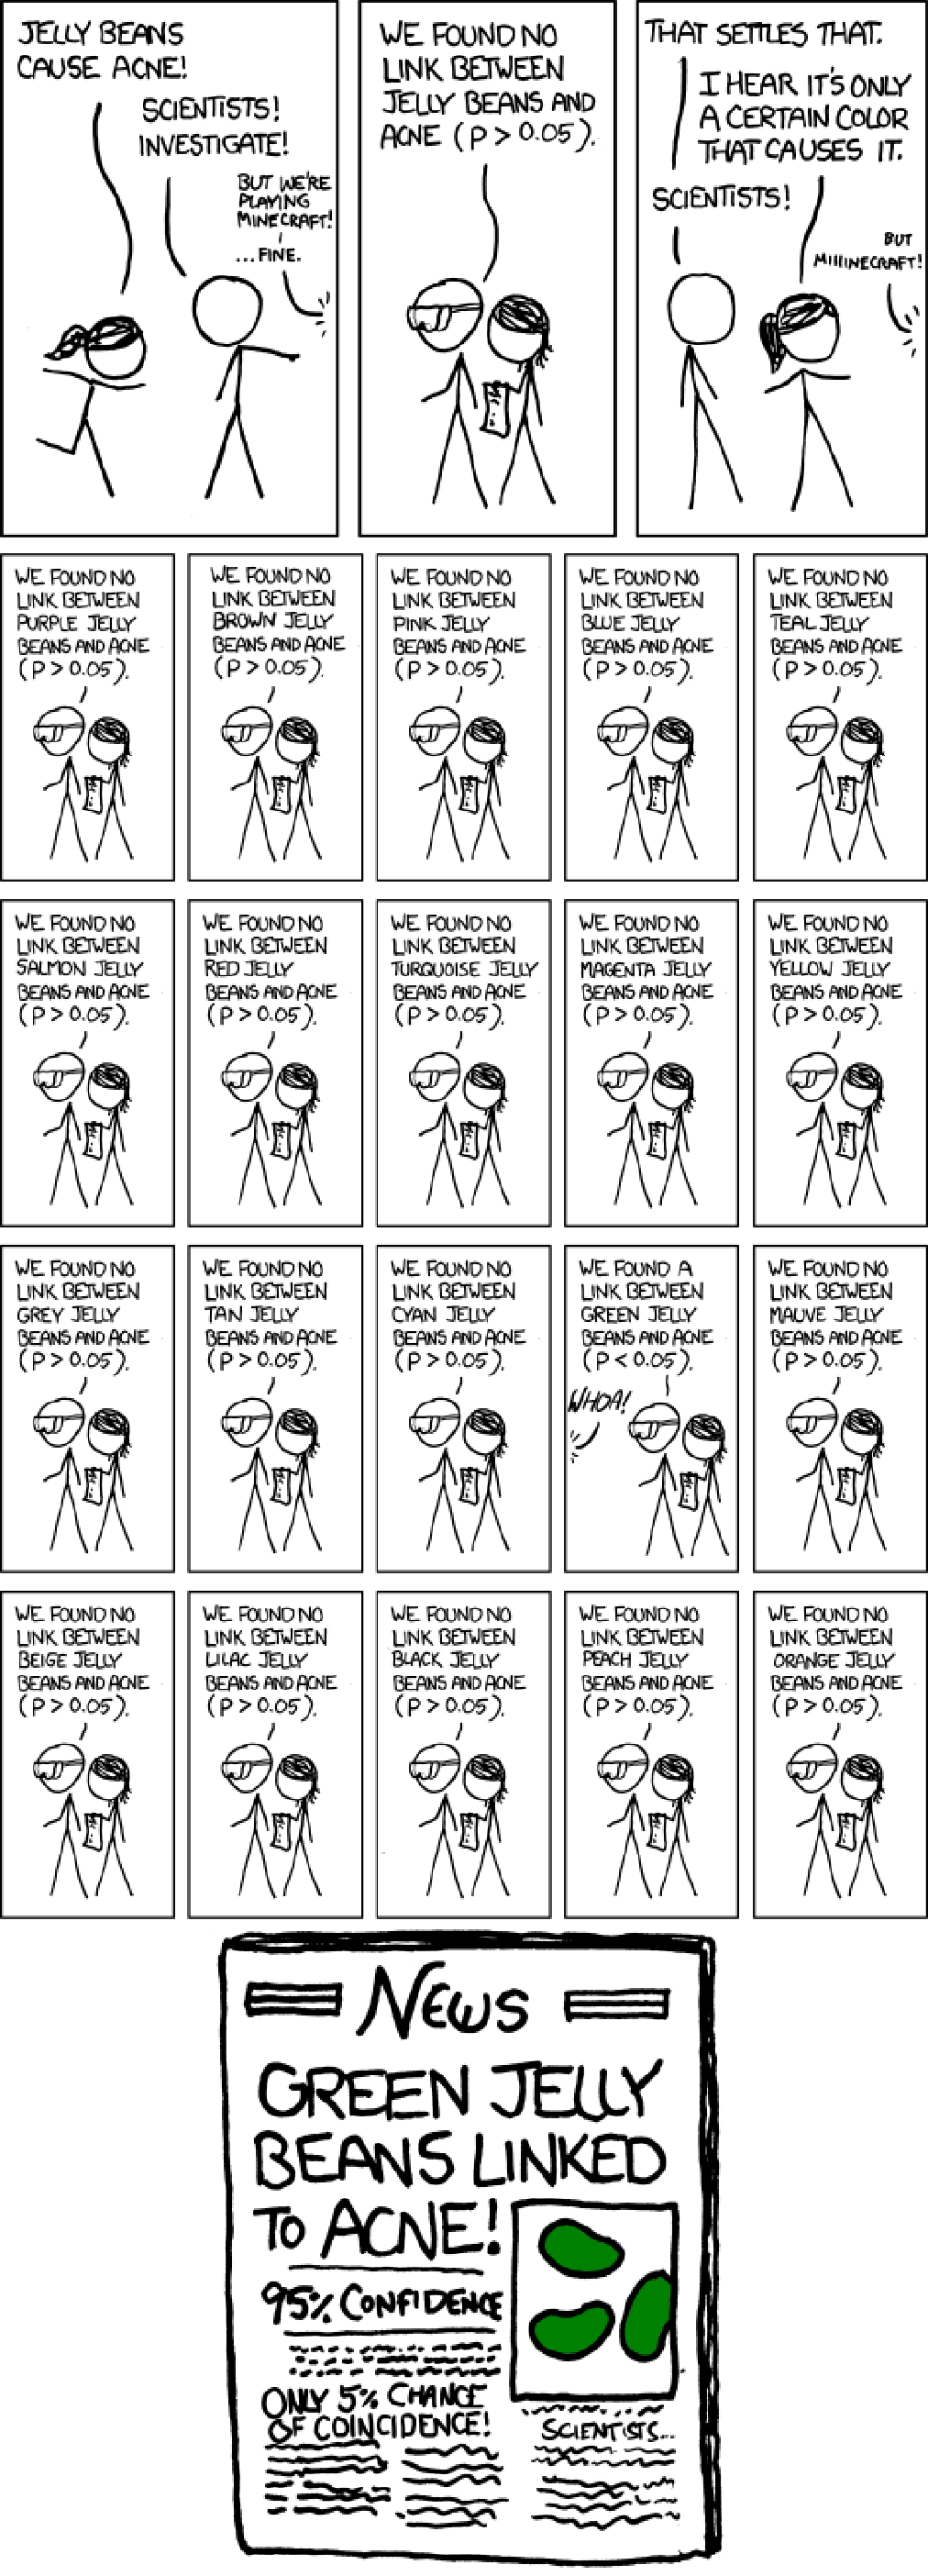
\includegraphics[width=8cm]{significant.eps}

            \fi

            \url{http://xkcd.com/882/}, image publiée sous licence \href{http://xkcd.com/license.html}{CreativeCommons}.

\end{center}

%+++++++++++++++++++++++++++++++++++++++++++++++++++++++++++++++++++++++++++++++++++++++++++++++++++++++++++++++++++++++++++ 
\section{Population et échantillon}
%+++++++++++++++++++++++++++++++++++++++++++++++++++++++++++++++++++++++++++++++++++++++++++++++++++++++++++++++++++++++++++

Pour reprendre le cas de l'acné, nous considérons la population française totale (65 millions de personnes), et nous voulons savoir si les \emph{jelly bean} sont liés à l'acné.

Il n'est évidemment pas question de tester toute la France. L'étude est en plusieurs étapes.
\begin{enumerate}
    \item
        On va demander aux spécialistes quel est le pourcentage de français souffrant d'acné. Disons pour l'exemple que le résultat soit de \( 20\%\).
    \item
        On prend un échantillon de français (disons \( 1000\)) mangeant régulièrement des \emph{jelly beans}, et on compte combien ont de l'acné.
    \item
        Si plus de \( 20\%\) des personnes de l'échantillon présente de l'acné, alors on se pose des questions.
\end{enumerate}

Dans l'échantillon, nous nous attendons à avoir 
\begin{equation}
    \frac{ 20 }{ 100 }\times 1000=200
\end{equation}
personnes développant de l'acné si les \emph{jelly beans} ne sont pas liées à l'acné. 

Évidemment, si on en a \( 201\) ou \( 199\), ce n'est pas un problème. La question précise à laquelle nous devons répondre est :
\begin{Aretenir}
    À partir de combien de personnes développant de l'acné, pouvons-nous dire que ça ne peut pas être le fruit du hasard ?
\end{Aretenir}
Et c'est la réponse à cette questions que ne connaît manifestement pas le journaliste qui a écrit l'article en fin de blague.

Le résultat-clef est le suivant.
\begin{Aretenir}
    Soit une population dans laquelle une proportion \( p\) d'individus présentent une certaine caractéristique. Soit aussi un échantillon de taille \( n\) prélevé au hasard dans cette population. Nous notons \( f\) la fréquence des individus de l'échantillon présentant la caractéristique. 

    Si \( p\) est encore \( 0.2\) et \( 0.8\) et si \( n\geq 30\), alors il y a \( 95\%\) de chances que 
    \begin{equation}
        f\in\mathopen[ p-\frac{1}{ \sqrt{n} } ; p+\frac{1}{ \sqrt{n} } \mathclose].
    \end{equation}
    Cet intervalle est appelé \defe{intervalle de fluctuation}{intervalle!de fluctuation} de l'échantillon.
\end{Aretenir}

Comment cela s'applique à notre étude de \emph{jelly bean} ? 
\begin{description}
    \item[Résumé des données]
        La proportion des français présentant de l'acné est dite de \( p=0.2\), et nous avons prélevé un échantillon de taille \( n=1000\). 
    \item[Intervalle de fluctuation] 
        Donc dans notre échantillon nous avons \( 95\%\) de chances que la fréquence soit dans l'intervalle
        \begin{equation}
            \mathopen[ 0.2-\frac{1}{ \sqrt{1000} } ; 0.2+\frac{1}{ \sqrt{1000} } \mathclose]\simeq\mathopen[ 0.168 ; 0.231 \mathclose]
        \end{equation}
        parce que \( \frac{1}{ \sqrt{1000} }\simeq 0.03162\).
    \item[Transformation en effectifs]

        Une fréquence de \( 0.168\) dans un échantillon de \( 1000\) individus revient à \( 168\) individus et une fréquence de \( 0.231\) revient à \( 231\) individus.

        Nous avons donc \( 95\%\) de chances que, en faisant l'étude sur \( 1000\) personnes, le nombre de personnes présentant de l'acné soit compris ente \( 168\) et \( 231\).
    \item[Décider si les \emph{jelly bean} provoquent l'acné]
        Si sur un échantillon de \( 1000\) personnes mangeant des \emph{jelly bean} nous en avons par exemple \( 260\) qui présentent de l'acné, alors nous pouvons dire que les \emph{jelly bean} sont liés à l'acné au sens où il y a moins de \( 5\%\) de chances que le résultats puisse s'expliquer par le hasard.

\end{description}

%+++++++++++++++++++++++++++++++++++++++++++++++++++++++++++++++++++++++++++++++++++++++++++++++++++++++++++++++++++++++++++ 
\section{Exercices}
%+++++++++++++++++++++++++++++++++++++++++++++++++++++++++++++++++++++++++++++++++++++++++++++++++++++++++++++++++++++++++++

\Exo{smath-0328}
